\section{图着色}
\label{sec:graph-coloring}

上一节的顶点标记细化给结构相似的顶点赋予相同的标记，用来比较两张图的邻域结构；本节讨论另一种给顶点赋标签的问题——要求任何两个相邻顶点都必须获得不同的标签（常称为“颜色”），并且使用的颜色种类越少越好。在第~\ref{sec:graph-cliques-independent-sets}小节中，单个独立集挑选出了一组彼此不冲突的顶点；如果我们需要把全部顶点都安排妥当，就必须把顶点集$V$划分为若干个互不相交的独立集，这正是图着色的任务。

\subsection{问题与思路}
\label{sec:graph-coloring-problem}

考试排课、无线基站信道分配或编译器寄存器分配中，每个顶点代表一门课程、一座基站或一个临时变量，每条边代表两门课程有共同选课学生、两座基站距离过近会产生同频干扰，或者两个变量的生命周期重叠而不能共用同一个寄存器。给每个顶点分配一个时段、一个频段或一个寄存器编号，就相当于给顶点涂上一种颜色：只要有边相连的两个顶点，颜色就绝不能相同。

\begin{definition}[正常顶点着色与色数]
\label{def:graph-vertex-coloring}
设$\mathcal G=(V,E)$是非空简单无向图，$k\geq 1$为整数。映射$c:V\to\{1,\ldots,k\}$若满足对每条边$\{u,v\}\in E$都有$c(u)\neq c(v)$，就称为$\mathcal G$的一个$k$-\term{正常顶点着色}（proper vertex coloring）。存在$k$-正常顶点着色的最小正整数$k$称为$\mathcal G$的\term{色数}（chromatic number），记作$\chi(\mathcal G)$。对空图另约定$\chi(\mathcal G)=0$。
\end{definition}

从顶点子集的结构来看，正常顶点着色与第~\ref{sec:graph-cliques-independent-sets}小节的独立集是一回事的两种说法。在正常顶点着色$c$下，取染第$r$种颜色的全部顶点组成颜色类
\[
V_r=\bigl\{v\in V:c(v)=r\bigr\}.
\]
由于相邻顶点颜色不同，$V_r$内部没有任何边，必是一个独立集。反过来，若把$V$划分为$k$个互不相交的独立集$V_1,\ldots,V_k$，给$V_r$中的顶点統一赋予颜色$r$，就得到一个$k$-正常顶点着色。因此，色数$\chi(\mathcal G)$恰好是把顶点集$V$划分为若干个独立集所需的最少块数。

这一等价性立即给出色数的两个基本结构下界：图中只要有一个大小为$\omega(\mathcal G)$的团，团内顶点两两相邻，就至少需要$\omega(\mathcal G)$种颜色；同时，每种颜色最多只能容纳$\alpha(\mathcal G)$个顶点，要覆盖全部$n$个顶点，颜色数至少为$n/\alpha(\mathcal G)$。

\begin{lemma}[色数的团数与独立数下界]
\label{lem:graph-chromatic-lower-bounds}
对任意有$n=|V|\geq 1$个顶点的简单无向图$\mathcal G=(V,E)$，其色数满足
\begin{equation}
\chi(\mathcal G)\geq\max\left\{\omega(\mathcal G),\,\left\lceil\frac{n}{\alpha(\mathcal G)}\right\rceil\right\}.
\label{eq:graph-chromatic-lower-bounds}
\end{equation}
\end{lemma}

\begin{proof}
设$K\subseteq V$是$\mathcal G$的一个最大团，$|K|=\omega(\mathcal G)$。由于$K$中任意两个不同顶点都相邻，任何正常顶点着色在$K$上必须取两两不同的颜色，故至少要用$\omega(\mathcal G)$种颜色，即$\chi(\mathcal G)\geq\omega(\mathcal G)$。

又设$V=V_1\cup\cdots\cup V_k$是$\mathcal G$取色数$k=\chi(\mathcal G)$时的颜色类划分。每个非空颜色类$V_r$都是独立集，故$|V_r|\leq\alpha(\mathcal G)$。对$r=1,\ldots,k$求和得
\[
n=\sum_{r=1}^{k}|V_r|\leq k\,\alpha(\mathcal G)=\chi(\mathcal G)\alpha(\mathcal G),
\]
两边除以$\alpha(\mathcal G)\geq 1$并取上整，即得$\chi(\mathcal G)\geq\lceil n/\alpha(\mathcal G)\rceil$。
\end{proof}

对非空图，特殊色数直接对应前面学过的特殊图结构。$\chi(\mathcal G)=1$当且仅当整张图本身就是一个独立集，即没有任何边（$m=0$）。当图至少有一条边时，$\chi(\mathcal G)=2$当且仅当$V$可以划分为两个独立集$V_1,V_2$，这正是第~\ref{sec:graph-bipartite-graphs}小节的二部图；第~\ref{sec:graph-bfs-bipartite}小节已经证明，利用广度优先遍历的层号奇偶性，可以在$O(n+m)$时间内判定是否有$\chi(\mathcal G)\leq 2$并给出具体的二着色。一旦图中出现奇环，例如五元环$C_5$，它不含三角形（$\omega(C_5)=2$），但五个顶点中最多只能选出两个不相邻顶点（$\alpha(C_5)=2$），由式\eqref{eq:graph-chromatic-lower-bounds}的第二个下界立知$\chi(C_5)\geq\lceil 5/2\rceil=3$，说明色数可以严格大于团数。

对于一般无向图，要直接穷举所有独立集划分来求最少颜色数是不可行的。构造正常顶点着色的基本思路是按某种次序$v_1,v_2,\ldots,v_n$逐个给顶点赋色：当处理到顶点$v_i$时，只需查看它在前面已经着色的邻居用掉了哪些颜色，然后贪心地挑出尚未被这些邻居占用的最小正整数颜色赋给$v_i$。

\subsection{算法实现}
\label{sec:graph-coloring-algorithm}

为了在邻接表上高效执行上述贪心规则，算法维护两项状态：
\begin{itemize}
  \item 颜色数组$c(\cdot)$：记录每个顶点$v$分配到的颜色编号$\{1,2,\ldots\}$，$0$表示尚未着色；
  \item 布尔标记数组$\operatorname{used}[1..\Delta(\mathcal G)+1]$：在处理当前顶点$v_i$时，临时标记哪些颜色已经被$v_i$的已着色邻居占用，初值全为假。
\end{itemize}

给定顶点排列$v_1,v_2,\ldots,v_n$后，外层循环按$i=1,\ldots,n$依次处理$v_i$：先扫描$v_i$的邻接表，对每个满足$c(u)\neq 0$的邻居$u$，将$\operatorname{used}[c(u)]$置为真；接着从$r=1,2,\ldots$向上查找第一个满足$\operatorname{used}[r]$为假的正整数$r$，置$c(v_i)=r$；最后再次扫描$v_i$的邻接表，把刚才置为真的$\operatorname{used}[c(u)]$还原为假，供下一个顶点使用。

\begin{algorithm}[贪心顶点着色算法]
\label{alg:graph-greedy-coloring}
输入：无向图$\mathcal G=(V,E)$的邻接表，顶点排列$v_1,v_2,\ldots,v_n$。输出：正常顶点着色$c(v)$。
\begin{enumerate}
  \item 初始化所有顶点$v\in V$的颜色$c(v)=0$，布尔数组$\operatorname{used}[1..n]$全为假。
  \item 对$i=1,2,\ldots,n$依次执行：
  \begin{enumerate}
    \item 扫描$v_i$的每个邻居$u\in N(v_i)$；若$c(u)>0$，置$\operatorname{used}[c(u)]\gets\text{真}$。
    \item 取使$\operatorname{used}[r]$为假的最小正整数$r\geq 1$，置$c(v_i)=r$。
    \item 再次扫描$v_i$的每个邻居$u\in N(v_i)$；若$c(u)>0$，置$\operatorname{used}[c(u)]\gets\text{假}$。
  \end{enumerate}
  \item 输出颜色数组$c(\cdot)$。
\end{enumerate}
\end{algorithm}

步骤2(c)只清理$v_i$邻居用过的颜色位置，而不把整个长度为$n$的$\operatorname{used}$数组全部清零；这样处理$v_i$的工作量就严格控制在与$1+d_{v_i}$成正比的范围之内。

\paragraph{顶点排序策略}
算法~\ref{alg:graph-greedy-coloring}总是输出合法的正常顶点着色，但所用颜色的总数依赖输入的顶点排列$v_1,\ldots,v_n$。以四点路径$P_4=(1,2,3,4)$（边集为$\{1,2\},\{2,3\},\{3,4\}$）为例，它是一棵树，也是二部图，真实色数为$\chi(P_4)=2$。若按自然顺序$(1,2,3,4)$着色（图~\ref{fig:graph-coloring-greedy}(b)），$1$染颜色$1$，$2$避开$1$染颜色$2$，$3$避开$2$染颜色$1$，$4$避开$3$染颜色$2$，只用$2$种颜色就达到最优。但若先把两个度为$1$的端点排在前面，按$(1,4,2,3)$的次序着色（图~\ref{fig:graph-coloring-greedy}(c)）：$1$染颜色$1$；接着处理$4$时，它的唯一邻居$3$尚未着色，于是$4$也染上了颜色$1$；随后处理$2$，它避开邻居$1$的颜色$1$而染颜色$2$；最后处理夹在中间的$3$，它的两个邻居$2$和$4$已经分别占用了颜色$2$和颜色$1$，迫使$3$启用第$3$种颜色。

为什么次序$(1,4,2,3)$会多用一种颜色？因为度较大的内部顶点$2,3$被留到了后面，等轮到它们时，周围互不相邻的邻居已经各自抢占了不同的颜色。为了减少这种被动冲突，实践中常采用两种排序策略：第一种是静态的按度递减次序（Welsh--Powell次序），预先按度数$d_{v_1}\geq d_{v_2}\geq\cdots\geq d_{v_n}$排列顶点，把邻居最多、受约束最强的顶点优先着色；第二种是动态的饱和度优先次序（DSATUR），每一步在尚未着色的顶点中，优先挑选“已着色邻居中包含不同颜色种类最多”（称为饱和度最大）的顶点着色，相同时再选度最大的顶点。在$P_4$上，这两种策略都会先处理度为$2$的内点$2,3$、再处理度为$1$的端点$1,4$，从而稳定地只用$2$种颜色。

\paragraph{执行过程}
在贯穿四点图\eqref{eq:graph-conn-running-graph}上，四个顶点的度依次为$2,3,3,2$。无论按编号顺序$(1,2,3,4)$还是按度递减顺序$(2,3,1,4)$执行算法~\ref{alg:graph-greedy-coloring}，都得到3-着色：按$(1,2,3,4)$执行时，$c(1)=1$；顶点$2$与$1$相邻，得$c(2)=2$；顶点$3$与$1,2$都相邻，$\operatorname{used}[1]$与$\operatorname{used}[2]$均为真，故$c(3)=3$；顶点$4$与$2,3$相邻，已着色邻居占用了颜色$2,3$，最小可用颜色为$1$，故$c(4)=1$（图~\ref{fig:graph-coloring-greedy}(a)）。所得的三个颜色类为$\{1,4\}$、$\{2\}$、$\{3\}$，所用颜色数$3$恰好等于最大团$\{1,2,3\}$给出的下界$\omega(\mathcal G)=3$，因此证实$\chi(\mathcal G)=3$。

\begin{figure}[!htb]
  \centering
  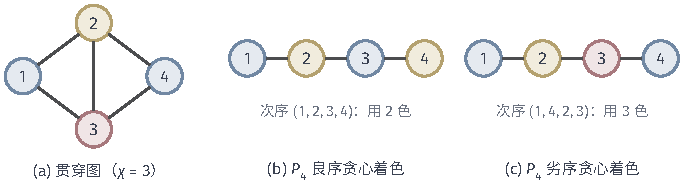
\includegraphics[width=115.761mm]{figures/03-graphs/01-structure-and-computation/tikz/graph-coloring-greedy/figure.pdf}
  \caption{贪心顶点着色及顶点次序的影响。蓝、黄、红分别表示颜色$1,2,3$。(a)贯穿图按$(1,2,3,4)$贪心着色，不相邻的$1,4$同染颜色$1$，共使用$3=\omega(\mathcal G)$种颜色，达到最优；(b)四点路径$P_4$按$(1,2,3,4)$依次着色，只用$2$种颜色；(c)同一条路径$P_4$若先给两端点$1,4$染同色$1$，再染$2,3$，则顶点$3$因邻居$2,4$已占用颜色$2,1$而被迫使用第$3$种颜色。}
  \label{fig:graph-coloring-greedy}
\end{figure}

\subsection{算法分析}
\label{sec:graph-coloring-analysis}

\paragraph{正确性与色数上界}
尽管不同的顶点次序可能改变贪心着色所用的颜色数，但无论按什么次序排列，所用颜色数都有一个只取决于最大度$\Delta(\mathcal G)=\max_{v\in V}d_v$的绝对上界。

\begin{theorem}[贪心着色的正确性与最大度上界]
\label{thm:graph-chromatic-bounds}
对任意有$n=|V|\geq 1$个顶点的简单无向图$\mathcal G=(V,E)$及任意顶点排列$v_1,\ldots,v_n$，算法~\ref{alg:graph-greedy-coloring}输出合法的正常顶点着色，且使用的颜色编号不超过$\Delta(\mathcal G)+1$。结合引理~\ref{lem:graph-chromatic-lower-bounds}，色数满足
\begin{equation}
\max\left\{\omega(\mathcal G),\,\left\lceil\frac{n}{\alpha(\mathcal G)}\right\rceil\right\}\leq \chi(\mathcal G)\leq \Delta(\mathcal G)+1.
\label{eq:graph-chromatic-bounds}
\end{equation}
\end{theorem}

\begin{proof}
对任一条边$\{v_i,v_j\}\in E$，不妨设在排列中$i<j$。当第$j$步给$v_j$赋色时，$v_i$已经着有正整数颜色$c(v_i)>0$，步骤2(a)将$\operatorname{used}[c(v_i)]$置为真，故步骤2(b)选出的颜色$c(v_j)$必不等于$c(v_i)$。因此每条边的两端颜色都不同，输出是正常顶点着色。

在第$i$步给$v_i$赋色时，$v_i$在全图中的邻居总数$d_{v_i}$不超过$\Delta(\mathcal G)$，故它在$\{v_1,\ldots,v_{i-1}\}$中的已着色邻居至多有$d_{v_i}\leq\Delta(\mathcal G)$个，步骤2(a)至多把$\operatorname{used}$数组中的$\Delta(\mathcal G)$个位置置为真。于是前$\Delta(\mathcal G)+1$个正整数$\{1,2,\ldots,\Delta(\mathcal G)+1\}$中至少有一个位置仍为假，步骤2(b)选出的最小可用颜色$r$必满足$r\leq\Delta(\mathcal G)+1$。这证明了$\chi(\mathcal G)\leq\Delta(\mathcal G)+1$。
\end{proof}

什么情况下色数$\chi(\mathcal G)$真的会达到上界$\Delta(\mathcal G)+1$？容易看出两类典型例子：一类是完全图$K_n$，每个顶点的度都是$\Delta(K_n)=n-1$，而$n$个顶点两两相邻，必须用$\chi(K_n)=n=\Delta(K_n)+1$种颜色；另一类是奇环$C_{2k+1}$，每个顶点的度都是$\Delta(C_{2k+1})=2$，而由定理~\ref{thm:graph-bipartite-odd-cycle}它不能二着色，必须用$\chi(C_{2k+1})=3=\Delta(C_{2k+1})+1$种颜色。

图论中著名的Brooks定理指出，对于连通简单无向图，这两类图就是仅有的例外：只要连通图$\mathcal G$既不是完全图也不是奇环，就有$\chi(\mathcal G)\leq\Delta(\mathcal G)$。这里引用该定理而不展开完整证明。仅把生成树的父节点排在子节点之后，还不足以证明这个更强的界：它能为每个非根顶点保留一个尚未着色的邻居，但根顶点仍需另外处理。

贯穿图\eqref{eq:graph-conn-running-graph}满足$\Delta(\mathcal G)=3$，它既不是完全图$K_4$也不是奇环，确实有$\chi(\mathcal G)=3\leq\Delta(\mathcal G)$。

\paragraph{复杂度}
在算法~\ref{alg:graph-greedy-coloring}的第$i$步中，步骤2(a)和步骤2(c)各扫描$v_i$的邻接表一次，耗时$O(d_{v_i})$；步骤2(b)从$r=1$向上查找第一个未标记的颜色，因为最多有$d_{v_i}$个颜色被标记为真，至多检查$d_{v_i}+1$个位置就必然遇到假，耗时也是$O(1+d_{v_i})$。对全部$n$个顶点累加，总工作量为
\[
\sum_{i=1}^{n}O(1+d_{v_i})=O(n+m),
\]
颜色数组和$\operatorname{used}$数组占$O(n)$额外空间。若预先采用按度递减的Welsh--Powell次序，由于顶点的度数都是$0$到$n-1$之间的整数，用桶排序（计数排序）可在$O(n)$时间内排好次序，总时间仍为$O(n+m)$。

\paragraph{适用范围与计算边界}
判定一张图能否用$k$种颜色正常着色（即$\chi(\mathcal G)\leq k$），在$k=2$与$k\geq 3$之间具有不同的计算复杂度。当$k=2$时，这等价于第~\ref{sec:graph-bfs-bipartite}小节的二部图判定：在一个连通分量中一旦固定起点的颜色，它的每个邻居在$\{1,2\}$中就只剩唯一的一种颜色可选，选择沿边唯一传播，不会产生分支，一次$O(n+m)$的广度优先遍历就能给出确切回答。

然而当$k=3$时，一个顶点染颜色$1$之后，它的每个邻居在$\{2,3\}$中都还有两种颜色可选。局部的选择不再唯一，不同分支上的颜色约束沿着环路在全图范围内相互制约，类似于第~\ref{sec:graph-euler-hamilton}小节中哈密顿圈面临的全局耦合：判断一般图是否满足$\chi(\mathcal G)\leq 3$已是NP完全问题。算法~\ref{alg:graph-greedy-coloring}的价值在于它能以$O(n+m)$的线性代价快速给出一个不超过$\Delta(\mathcal G)+1$色的可行方案；当问题要求严格最小化颜色数且图的规模较大时，则需要结合回溯搜索或整数规划进一步求解。
